\documentclass[12pt, a4paper]{article}

\usepackage{amssymb, amsmath}
\usepackage[utf8]{inputenc}
\usepackage{fullpage}
\usepackage{graphicx}
\usepackage{caption}
\usepackage{subcaption}
\usepackage{hyperref}
\usepackage{parskip}
\usepackage{url}


\author{Manuel Haid (1131404) \\ Thomas Mauerhofer (1031957) \\ Matthias Wölbitsch (1130899) \\ \\ Group 001}
\title{Project Plan for \texttt{timeline}: a Time Series Visualization Platform}
\date{}


\begin{document}


\maketitle


\section{Motivation}

In today's society data plays a import role in many different ways.
For instance, businesses are using large amount of data to predict consumer behavior to satisfy their demand.
Often time plays a essential role in these data sets. 
For example, the consumption of electricity does not only depend on the time of the day, but also on the day of the week and other seasonal effects.
Such data sets are usually referred to as time series (i.e. two- or higher-dimensional data with time as one dimension). 

When dealing with time series usually one of the first steps in the analysis process is the visualization of the data.
The graphical representation can already give some great insights in properties of the data.
For example, a simple visual inspection can show patterns, trends or seasonal effects without the use of advanced statistical methods. 
These properties are important since they have to be considered in the modeling of the time series (e.g. in forecasting models).
The goal of our project is to create a web-based platform that allows the user to perform this initial visual inspection of the time series in a convenient but sophisticated way.


\section{Project Description}

The time series visualization platform mainly consists of of a front-end and a back-end part.
This architectural design choice implies a clear separation of concerns. 
The back-end will be implemented in Python and is used for the processing of the data while the HTML/JavaScript front-end is used to present different views to the user.

One of the main responsibilities of the back-end application is the process of importing the data.
Currently we plan to provide three different ways to load data from an external source:

\begin{enumerate}
 \item \textbf{File import}: The most common way is a simple import of the data from files on the local file system.
 All supported import file formats are not specified yet, however, the usual formats such as \texttt{.csv} or \texttt{.tsv} should work with the application.
 \item \textbf{External APIs}: This import method could be used to easily explore data sets which are available on data set hosting sites. 
 For example, the well-known Time Series Data Library (TSDL) is hosted on \url{www.DataMarket.com} and could be accessed via an API. 
 \item \textbf{Sockets}: This import method could be used to explore data which is collected in real-time (e.g. sensor data). 
 However, further research is required to investigate the design of such interface for socket connections that provide data over time (e.g. sampling, \ldots).
\end{enumerate}

After the time series data was imported it should be stored in a appropriate data model. 
For this task we'll use the data analysis library pandas since it provides convenient high-performance data structures to store, access, and manipulate the data.
Other advantages of pandas are the support of operations on temporal data (e.g. slicing, filtering, \ldots) and the support of other libraries (e.g. NumPy) for pandas data structures.

Another important part of the back-end is the visualization engine. 
Its main responsibility is the processing of the time series to create visualization primitives (i.e. it transforms the data stored in the model into representations that can later be rendered by the front-end).
The visualization engine provides a RESTful API for its functionality, which is another part of the back-end.
This allows the front-end to send simple HTTP requests to get visualization primitives of the time series.
To implement the API we'll use the Flask microframework which makes things like RESTful request dispatching quite easy.

The front-end of the application is a simple HTML5 website that uses a JavaScript visualization library to display the visualization primitives.
Which library will be used was not decided yet.
However, a little bit of research showed that there plenty of different libraries available that support the plotting of temporal data.
For example, two time series visualization libraries, that are based on the well-known D3.js libary, are Cubism.js and MetricsGraphics.js could be used for this project.
Currently we plan to support the following visualization primitives which can be generated by the visualization engine and rendered by the front-end:

\begin{enumerate}
 \item Simple time series graphs, which plot the observations (i.e. the data points) against the time of the observations.
 \item Filtered time series graphs, which allow the user to select data in a certain time span or with other distinct attributes.
 \item Possibility to show multiple different time series in the same figure or in linked figures (see \autoref{fig:time_series_plots}).
 \item Possibility to show the running average and running standard deviation of a time series in a time graph (used to determine stationarity of a time series).
 \item Time series graphs which are live updated whenever new data is available on a socket (i.e. live visualization of a time series).
 \item Seasonal plots (i.e. plots in which the data is plotted against the individual season in which it was observed).
 \item Autocorrelation function (ACF) plots, which are a statistical tool to proof seasonal effects in the data (see \autoref{fig:acf}).
 \item Forecasting model evaluation plots that highlight three different parts of model in a time series graph:
 \begin{enumerate}
  \item The section of the time series that was used as training data for the model.
  \item The forecasted time series including a confidence interval up to the horizon of the prediction.
  \item The real values of the time series for the forecasted interval if available.
 \end{enumerate}
\end{enumerate}

\begin{figure}[ht!]
  \centering
  \begin{subfigure}[b]{0.45\textwidth}
    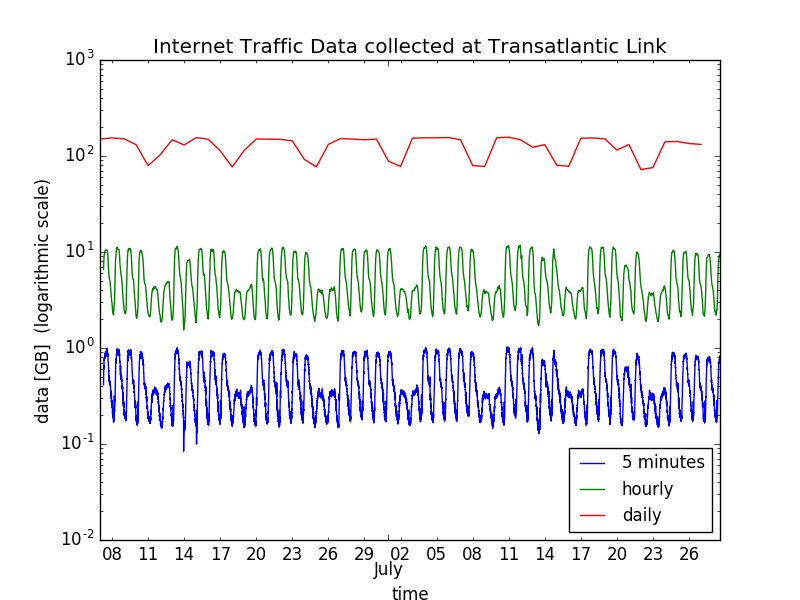
\includegraphics[width=\textwidth]{images/timeplot.png}
    \caption{Exemplary time series plot that shows three different data sets.}
    \label{fig:time_series_plots}
  \end{subfigure}
  ~
  \begin{subfigure}[b]{0.45\textwidth}
    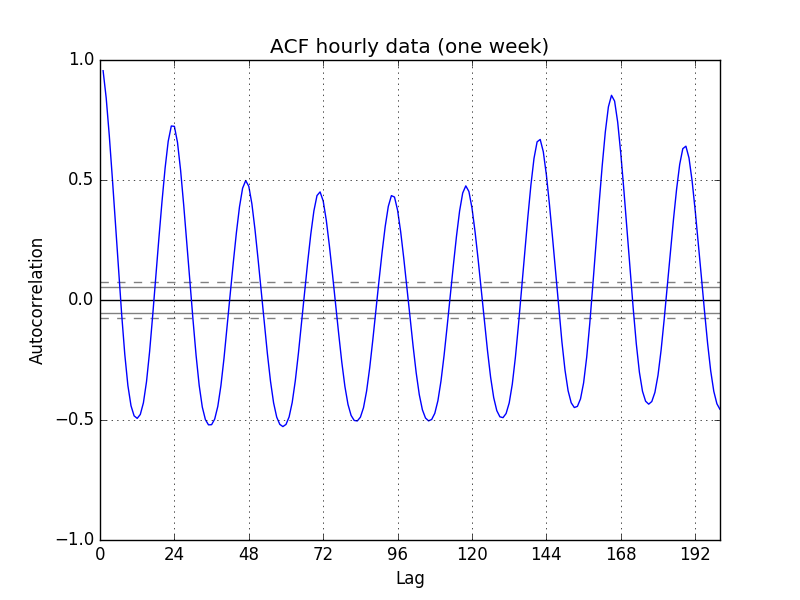
\includegraphics[width=\textwidth]{images/acf.png}
    \caption{An exemplary autocorrelation function plot that shows seasonal patterns.}
    \label{fig:acf}
  \end{subfigure}
  \caption{Examples for different visualizations of time series.}
\end{figure}


\section{Timetable}

\autoref{tab:timetable} shows some time estimates for the duration of different tasks from various areas of the project. 

\begin{table}[ht!]
\centering
\begin{tabular}{|l|c|}
\hline
\multicolumn{1}{|c|}{\textbf{Task}} & \textbf{Duration [h]} \\ \hline
\textbf{Research} &  \\ \hline
  - File import & 3 \\ \hline
  - APIs & 5 \\ \hline
  - Sockets & 10 \\ \hline
  - Python libraries & 5 \\ \hline
  - JavaScript visualization libraries & 5 \\ \hline
\textbf{Implementation} &  \\ \hline
  - User interface & 10 \\ \hline
  - Import model & 5 \\ \hline
  - Communication with APIs & 10 \\ \hline
  - Sockets & 15 \\ \hline
  - Generation of visualization primitives & 10 \\ \hline
  - Visualization & 15 \\ \hline
\textbf{Documentation} &  \\ \hline
  - Code & 2 \\ \hline
  - Projectplan & 10 \\ \hline
  - Report & 10 \\ \hline
\end{tabular}
\caption{Estimation for various sub tasks of the project.}
\label{tab:timetable}
\end{table}


\section{Responsibilities}

\begin{description}
 \item[Manuel Haid]: user interface, import model
 \item[Thomas Mauerhofer]: communication with APIs, visualization 
 \item[Matthias Wölbitsch]: generation of visualization primitives, sockets
\end{description}


\end{document}
